Let's now continue with the factorization journey. We have said in the introduction of types of factorizations that, given $A \in \mathbb{R}^{n\times n}$, we have:
\[
    A = X \Lambda X^{-1}
\]
Where $X$ has as columns the eigenvectors of A, while $\Lambda$ is a diagonal matrix with the eigenvalues of $A$ on the diagonal. Now, let's consider the case where the matrix $S$ is symmetric.
\[
    S \in \mathbb{R}^{n\times n} \hspace{1cm} S = S^\intercal
\]
We can factorize $S$ as follows:
\[
    S = Q \Lambda Q^\intercal
\]
Where $Q$ is orthogonal (this is true only because $S$ is symmtric) and $\Lambda$ is diagonal.
We can prove that $Q$ is orthogonal by:
\begin{enumerate}
    \item Consider the two vectors $\underline{x}, \underline{y}$ such as: $S\underline{x} = \lambda\underline{x}$ and $S\underline{y} = 0\underline{y}$. So, we are saying that both vectors are eigenvectors.
    \[
        \begin{rcases}
            \underline{y} \in N(S)\\
            \underline{x} \in \mathcal{C}(S) = \mathcal{C}(S^{\intercal})    
        \end{rcases}
        \implies \underline{x} \perp \underline{y}
    \]
    This is confirmed also by the scheme done during lecture with the 4 blocks. Notice that we have not specified or made any assumption on the value of $\lambda$.
    \item Similar to point 1, we consider the two vectors $\underline{x}, \underline{y}$ such as: $S\underline{x} = \lambda\underline{x}$ and $S\underline{y} = \alpha\underline{y}$. Now, consider the matrix $(S - \alpha I)$, we can write:
    \[
        (S - \alpha I)\underline{y} = 0\underline{y} \implies \underline{y} \in N(S - \alpha I)
    \]
    \[
        (S - \alpha I)\underline{x} = (\lambda - \alpha)\underline{x} \implies \underline{x} \in \mathcal{C}(S - \alpha I) = \mathcal{C}((S - \alpha I)^{\intercal})
    \]
    So, again we obtain: $\underline{x} \perp \underline{y}$.
\end{enumerate}
There is another property: $\lambda_i \in \mathbb{R}$, so the eigenvalues on the diagonal of $\Lambda$ are real. Proof:
\[
    S\underline{x} = \lambda\underline{x} \implies \overline{\underline{x}}^\intercal S\underline{x} = \lambda\overline{\underline{x}}^\intercal\underline{x}     
\]
The $\overline{\underline{x}}$ represent the conjugate of the vector $\underline{x}$. If that vector has complex components, those elements are conjugated, otherwise, i.e. they are all real, they remain inalterated. In particular, once a complex number is conjugated, the result is a real number, as shown here:
\[
    (a + ib)(a - ib) = (a^2 + b^2) \in \mathbb{R}    
\]
From the previos equation, we obtain:
\[
    \lambda = \frac{\overline{\underline{x}}^\intercal S\underline{x}}{\overline{\underline{x}}^\intercal\underline{x}} \in \mathbb{R}
\]

\subsection{Positive-definite symmetric matrices (SPD)}
Characterizations:
\begin{enumerate}[i]
    \item $\lambda_i > 0 \hspace{0.5cm} \forall i = 1, \dots, n$
    \item $\underline{v}^\intercal S \underline{v} \geq 0 \hspace{0.5cm} \forall \underline{v} \in \mathbb{R}^n$, with equality if and only if $\underline{v} = 0$
    \item Leading determinants are positive. \\
    \begin{multicols}{2}
        \begin{center}
            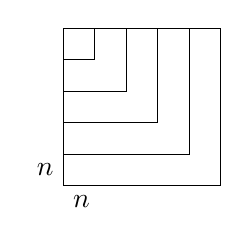
\begin{tikzpicture}
                \draw (0,0) -- (2,0) -- (2,2) -- (0,2) -- (0,0);
                \draw (0,0.4) -- (1.6,0.4) -- (1.6,2) -- (0,2) -- (0,0);
                \draw (0,0.8) -- (1.2,0.8) -- (1.2,2) -- (0,2) -- (0,0); 
                \draw (0,1.2) -- (0.8,1.2) -- (0.8,2) -- (0,2) -- (0,0) node[above left]{$n$};
                \draw (0,1.6) -- (0.4,1.6) -- (0.4,2) -- (0,2) -- (0,0) node[below right]{$n$};
            \end{tikzpicture}
        \end{center}

        This means that the determinant of the matrix obtained by taking the first $k$ rows and columns of $S$ is positive, $\forall k = 1, \dots, n$.
    \end{multicols}

    \item Cholesky decomposition: $S = B^\intercal B$, with $B$ upper triangular
    \item All pivot elements are positive in the Gaussian elimination process
\end{enumerate}

Let's consider $\lambda > 0$ being a certain eigenvalue. 
\[ 
    S\underline{x} = \lambda\underline{x}    
\]
We multiply both sides by $\underline{x}^\intercal$:
\[
    \underline{x}^\intercal S\underline{x} = \lambda\underline{x}^\intercal\underline{x} = \lambda\||\underline{x}\||^2 \geq 0
\]
Recall that $\underline{x}$ is an eigenvector while the before considered vector $\underline{v}$ is a generic vector. With $\underline{v}$, instead, we have:
\[
    \underline{v} = (c_1\underline{x}_1 + c_2\underline{x}_2 + \dots + c_n\underline{x}_n)    
\]
So we are expressing $\underline{v}$ as a linear combination of the eigenvectors of $S$. 
\[
    (c_1\underline{x}_1 + c_2\underline{x}_2 + \dots + c_n\underline{x}_n)^\intercal S (c_1\underline{x}_1 + c_2\underline{x}_2 + \dots + c_n\underline{x}_n)        
\]
\[
    \begin{rcases}
        c_1^2\underline{x}_1^\intercal S \underline{x}_1 = c_1^2\lambda_1\underline{x}_1^\intercal \underline{x}_1 = c_1^2\lambda_1||\underline{x}_1||^2\\
        c_1c_2\underline{x}_1^\intercal S \underline{x}_2 = c_1c_2\lambda_2\underline{x}_1^\intercal \underline{x}_2 = 0\\
    \end{rcases}    
    \text{there are two types of components}
\]
The first components is given by the eigenvectors with the same direction, while the second no so their scalar product is null (they are orthogonal).\\

From \textit{iv}):
\[
    S = B^\intercal B \implies \underline{v}^\intercal(B^\intercal B)\underline{v} = (\underline{v}^\intercal B^\intercal)(B \underline{v}) = (B\underline{v})^\intercal (B\underline{v}) = ||B\underline{v}||^2 \geq 0   
\]

\section{Singular Value Decomposition (SVD)}
We are going to use it for:
\begin{itemize}
    \item Least-squares approximation by introducing the pseudo-inverse of a matrix (Moore-Penrose inverse)
    \item Low-rank approximation with the Eckart-Young theorem
\end{itemize}
We start from:
\[
A \in \mathbb{R}^{m \times n} \hspace{1cm} 
\begin{cases}
m = \text{\# of samples}\\
n = \text{\# of features}
\end{cases}    
\]
We can write:
\[
    A = U\Sigma V^\intercal    
\]
With:
\begin{itemize}
    \item $U$ with dimensions $m \times m$ and orthogonal
    \item $V^\intercal$ with dimensions $n \times n$ and orthogonal
    \item $\Sigma$ with dimensions $m \times n$ \textit{almost} diagonal
\end{itemize}
If $m > n$, we can represent the matrices like this:
\[
\underbrace{
  \begin{bmatrix}
    & & & & & \\
    & & & & & \\
    & & & & & \\
    & & & & & \\
    & & & & & \\
  \end{bmatrix}}_{m \times m}
\underbrace{
  \begin{bmatrix}
    & & & \\
    & & & \\
    & & & \\
    & & & \\
    & & & \\
  \end{bmatrix}}_{m \times n}
\underbrace{
  \begin{bmatrix}
    & & & \\
    & & & \\
    & & & \\
  \end{bmatrix}}_{n \times n}
\]
What is the idea of SVD? Try to change features so variances are maximized and covariances are minimized. We don't want columns to be correlated.\\

In general: rank($A$) = $r < n$.
\[
    AV = U\Sigma \impliedby V^\intercal V = I \impliedby V \text{ is orthogonal}    
\]
The component wise notation is:
\[
    A\underline{v_i} = \sigma_i\underline{u_i}    
\]
Given that the rank of $A$ is $r$:

\[
\begin{bmatrix}
    & & & & & & &\\
    & & & & & & &\\
    & & & & & & &\\
    & & & & & & &\\
    & & & & & & &\\
    & & & & & & &\\
\end{bmatrix}
\begin{bmatrix}
    \sigma_1 & & & &\\
    & \sigma_2 & & &\\
    & & \ddots & &\\
    & & & \sigma_r &\\
    & & & & 0\\
    \hline
    0 & 0 & 0 & 0 & 0\\
    0 & 0 & 0 & 0 & 0\\
\end{bmatrix}
\begin{bmatrix}
    & & & & \\
    & & & & \\
    & & & & \\
    & & & & \\
\end{bmatrix}
\hspace{1cm}
\begin{cases}
\sigma_1, \dots, \sigma_r > 0\\
\sigma_{r+1}, \dots, \sigma_n = 0
\end{cases}  
\]
Typically: $\sigma_1 > \sigma_2 > \dots > \sigma_r > \sigma_{r+1} = 0$.
We have:
\[
\begin{cases}
    \begin{rcases}
        A\underline{v_1} = \sigma_1\underline{u_1}\\
        \hspace{1cm}\vdots\\
        A\underline{v_r} = \sigma_r\underline{u_r}\\        
    \end{rcases} r\\
    \begin{rcases}
        A\underline{v_{r+1}} = \sigma_{r+1}\underline{u_{r+1}}\\
        \hspace{1cm}\vdots\\
        A\underline{v_n} = \sigma_n\underline{u_n}\\        
    \end{rcases} n-r
\end{cases}    
\]
So the first $r$ vectors span the column space of $A$ while for the last $n-r$ means that $\underline{v_i} \in N(A)$ for $i = r+1, \dots, n$.
If we have $A^\intercal$, the decomposition is $A^\intercal = (U\Sigma V^\intercal)^\intercal = V\Sigma^\intercal U^\intercal$. 

\subsection{Economy SVD}
What we've seen so far is the full SVD, but it can be optimized. Here is following the compact (reduced) representation, where once again we consider $m > n$:
\[
\underbrace{
  \begin{bmatrix}
    & & & \\
    & & & \\
    & & & \\
    & & & \\
    & & & \\
  \end{bmatrix}}_{m \times n}
\underbrace{
  \begin{bmatrix}
    & & & \\
    & & & \\
    & & & \\
  \end{bmatrix}}_{n \times n}
\underbrace{
  \begin{bmatrix}
    & & & \\
    & & & \\
    & & & \\
  \end{bmatrix}}_{n \times n}
\]
This is caused by the fact that the last $m-n$ rows in the central matrix are all 0 so multiply them for the last $m-n$ columns of the left matrix is useless. This can be furthermore optimized by having matrix dimensions: $(m\times r)(r\times r)(r\times n)$ because not all $\sigma$ might be different than 0 (i.e. the rank of $A$ is $r$), so, in that case is useless even to multiply the last $m-r$ rows of the central matrix. \\

\textbf{The SVD works for any matrix $A$.}\\

\noindent Let's suppose $A$ is full rank $n\times n$:
\[
    A = U\Sigma V^\intercal = \sum_{i = 1}^{n} \sigma_i \underbrace{\underline{u_i}\underline{v_i}^\intercal}_{\text{rank }=1}    
\]
View matrix-matrix multiplication for the rank 1 concept.
If $A$ is not full rank but instead has rank($A$)=$r$, the same sum is nomore computed until $n$, but instead $r$.
\[
    A = \sum_{i = 1}^{r} \sigma_i \underline{u_i}\underline{v_i}^\intercal   
\]
What happens now if we pick a certain value $\tilde{r} < r$?
\[
    A = U\Sigma V^\intercal \cong \sum_{i = 1}^{\tilde{r}} \sigma_i \underline{u_i}\underline{v_i}^\intercal   
\]
We obtain a \textbf{rank $\tilde{r}$ approximation of the matrix A}. The rank of the matrix is know because is the sum of $\tilde{r}$ matrices of rank 1. Moreover, that one, is the best approximation of rank $\tilde{r}$ possible, i.e.:
\[
    ||A - \tilde{A}|| \leq ||A - B|| \hspace{1cm} \forall B  \text{ of rank} = \tilde{r}    
\]

\subsection{Proof of the existence of SVD}
Once again, we start from matrix $A \in \mathbb{m \times n}$ an rank$=r$. We consider the new matrix $A^\intercal A$ which is:
\begin{itemize}
    \item symmetric: $(A^\intercal A)^\intercal = A^\intercal A$
    \item positive definite: $\underline{x}^\intercal(A^\intercal A)\underline{x} = (\underline{x}^\intercal A^\intercal)(A \underline{x}) = (A\underline{x})^\intercal (A\underline{x}) = ||A\underline{x}||^2 \geq 0  $
\end{itemize} 
We can use the following decomposition:
\[
    A^\intercal A = V\Lambda V^\intercal = \sum_{i=1}^n \lambda_i \underline{v_i} \underline{v_i^\intercal}    
\]
Recall that $V$ contains the eigenvectors while $\Lambda$ contains the eigenvalues. We rename $\lambda_i = \sigma_i^2$. The rank of $A^\intercal A$ is $r$.\\

We want to prove that if  $\underline{x} \in N(A)$ then $\underline{x} \in N(A^\intercal A)$, to do so we proceed in both directions:
\begin{enumerate}
    \item If we have $A\underline{x} = 0 \implies \underline{x} \in N(A)$. Is it possible to multiply both terms:
    \[
        A^\intercal(A\underline{x}) = A^\intercal \underline{0} = \underline{0} \hspace{1cm} \text{so} \hspace{1cm} \underline{x} \in N(A) \implies \underline{x} \in N(A^\intercal A)
    \]
    \item We start from $(A^\intercal A)\underline{x} = 0 \implies \underline{x} \in N(A^\intercal A)$. Again, we multiply:
    \[
        \underline{x}^\intercal A^\intercal A\underline{x} = ||A\underline{x}||^2 = 0 \hspace{1cm} \text{so} \hspace{1cm} \underline{x} \in N(A^\intercal A) \implies \underline{x} \in N(A)
    \]
\end{enumerate}
Let's consider the couple of (eigenvalues, eigenvectors) = ($\sigma_i^2, \underline{v_i}$):
\[
    A^\intercal A\underline{v_i} = \sigma_i^2 \underline{v_i} \hspace{0.3cm}\overset{\text{component-wise}}{\longrightarrow} \hspace{0.3cm} A^\intercal A\underline{v_i} = \sigma_i^2 \underline{v_i} \hspace{1cm} (\dagger)
\]
We introduce the quantity $\underline{u_i} = \dfrac{A\underline{v_i}}{\sigma_i}$ which has some characteristics:
\begin{enumerate}[i]
    \item $\underline{u_i}$ are unitary vectors:
    \[
        \underline{u_i}^\intercal \underline{u_i} = \left(\dfrac{A\underline{v_i}}{\sigma_i}\right)^\intercal \left(\dfrac{A\underline{v_i}}{\sigma_i}\right) = \dfrac{\underline{v_i^\intercal}A^\intercal A\underline{v_i}}{\sigma^2} \overset{\dagger}{=} \dfrac{\sigma_i^2 \underline{v_i^\intercal}\underline{v_i}}{\sigma_i^2} = 1
    \]
    The last passage of the equation is true because $\underline{v_i}$ vectors are orthonormal.
    \item $\underline{u_i} \perp \underline{u_j}$:
    \[
        \underline{u_i}^\intercal \underline{u_j} = \left(\dfrac{A\underline{v_i}}{\sigma_i}\right)^\intercal \left(\dfrac{A\underline{v_j}}{\sigma_j}\right) = \dfrac{\underline{v_i^\intercal}A^\intercal A\underline{v_j}}{\sigma_i \sigma_j} \overset{\dagger}{=} \dfrac{\sigma_j^2 \underline{v_i^\intercal}\underline{v_j}}{\sigma_i \sigma_j} = 0
    \] 
    \item $\underline{u_i}$ are eigenvectors of $AA^\intercal$ with eigenvalues $\sigma_i^2$:
    \[
        (AA^\intercal \underline{u_i}) = AA^\intercal\left(\dfrac{A\underline{v_i}}{\sigma_i}\right) = A\dfrac{A^\intercal A\underline{v_i}}{\sigma_i} \overset{\dagger}{=} A\dfrac{\sigma_i^2 \underline{v_i}}{\sigma_i} = \sigma_i^2\left(\dfrac{A\underline{v_i}}{\sigma_i}\right) = \sigma_i^2\underline{u_i}   
    \]
\end{enumerate}
We have demonstrated that $A\underline{u_i} = \sigma_i \underline{u_i}$ and $\underline{u_i}$ are orthonormal as well. 